% ---------------------------------------------------------------------
%  MarketSage AI --- standalone part PDF
%  Auto-generated wrapper. Content lives in parts/05_event_engine.tex
%  Build: pdflatex part05.tex   (run twice)
% ---------------------------------------------------------------------
% =====================================================================
%  MarketSage AI  --  Master Engineering & Strategy Blueprint
%  Author: Aditya Sikarwar
%  Compile:  pdflatex marketsage_master_plan.tex   (run twice for TOC)
% =====================================================================
\documentclass[11pt,a4paper]{report}

\usepackage[T1]{fontenc}
\usepackage[utf8]{inputenc}
\usepackage{lmodern}
\usepackage[margin=2.2cm,top=2.4cm,bottom=2.4cm]{geometry}
\usepackage{amsmath,amssymb}
\usepackage{graphicx}
\usepackage{xcolor}
\usepackage{booktabs}
\usepackage{longtable}
\usepackage{array}
\usepackage{multirow}
\usepackage{enumitem}
\usepackage{fancyhdr}
\usepackage{titlesec}
\usepackage{tikz}
\usepackage{listings}
\usepackage{tcolorbox}
\usepackage[hidelinks]{hyperref}

\usetikzlibrary{positioning,arrows.meta,shapes.geometric,calc,fit,backgrounds}
\tcbuselibrary{skins,breakable}

% ---------------------------------------------------------------- colours
\definecolor{msblue}{HTML}{0B3D91}
\definecolor{mscyan}{HTML}{0E7C86}
\definecolor{msamber}{HTML}{B26A00}
\definecolor{msred}{HTML}{9B1C1C}
\definecolor{msgreen}{HTML}{1B5E20}
\definecolor{msgrey}{HTML}{4A4A4A}
\definecolor{mslight}{HTML}{EEF3FA}
\definecolor{msline}{HTML}{C8D4E4}

% ---------------------------------------------------------------- headers
\pagestyle{fancy}
\fancyhf{}
\renewcommand{\headrulewidth}{0.4pt}
\fancyhead[L]{\footnotesize\textsc{MarketSage AI}}
\fancyhead[R]{\footnotesize\leftmark}
\fancyfoot[C]{\footnotesize\thepage}

\titleformat{\chapter}[display]
  {\normalfont\Huge\bfseries\color{msblue}}
  {\normalsize\color{msgrey}\MakeUppercase{\chaptertitlename}\ \thechapter}{6pt}{\Huge}
\titlespacing*{\chapter}{0pt}{-18pt}{22pt}
\titleformat{\section}{\normalfont\Large\bfseries\color{msblue}}{\thesection}{0.7em}{}
\titleformat{\subsection}{\normalfont\large\bfseries\color{mscyan}}{\thesubsection}{0.6em}{}

% ---------------------------------------------------------------- boxes
\newtcolorbox{keybox}[1][]{
  enhanced,breakable,colback=mslight,colframe=msblue,
  boxrule=0.7pt,left=7pt,right=7pt,top=8pt,bottom=6pt,
  fonttitle=\bfseries\color{white},coltitle=white,
  colbacktitle=msblue,attach boxed title to top left={xshift=8pt,yshift=-8pt},
  boxed title style={boxrule=0pt,arc=1pt},#1}

\newtcolorbox{warnbox}[1][]{
  enhanced,breakable,colback=red!3,colframe=msred,
  boxrule=0.7pt,left=7pt,right=7pt,top=8pt,bottom=6pt,
  fonttitle=\bfseries\color{white},coltitle=white,
  colbacktitle=msred,attach boxed title to top left={xshift=8pt,yshift=-8pt},
  boxed title style={boxrule=0pt,arc=1pt},#1}

\newtcolorbox{gatebox}[1][]{
  enhanced,breakable,colback=green!3,colframe=msgreen,
  boxrule=0.7pt,left=7pt,right=7pt,top=8pt,bottom=6pt,
  fonttitle=\bfseries\color{white},coltitle=white,
  colbacktitle=msgreen,attach boxed title to top left={xshift=8pt,yshift=-8pt},
  boxed title style={boxrule=0pt,arc=1pt},#1}

% ---------------------------------------------------------------- listings
\lstdefinestyle{ms}{
  basicstyle=\ttfamily\scriptsize,
  keywordstyle=\color{msblue}\bfseries,
  commentstyle=\color{msgrey}\itshape,
  stringstyle=\color{mscyan},
  numbers=left,numberstyle=\tiny\color{msgrey},
  frame=single,rulecolor=\color{msline},
  breaklines=true,showstringspaces=false,
  backgroundcolor=\color{mslight},
  columns=fullflexible
}
\lstset{style=ms}

% ---------------------------------------------------------------- tikz styles
\tikzset{
  blk/.style={rectangle,rounded corners=3pt,draw=msblue,fill=mslight,
              text width=2.6cm,align=center,inner sep=5pt,font=\scriptsize},
  wide/.style={rectangle,rounded corners=3pt,draw=msblue,fill=mslight,
              text width=3.25cm,align=center,inner sep=5pt,font=\scriptsize},
  lay/.style={rectangle,rounded corners=4pt,draw=msblue!60,fill=white,
              inner sep=8pt},
  ar/.style={-{Stealth[length=2.5mm]},draw=msblue,thick},
  arg/.style={-{Stealth[length=2.5mm]},draw=mscyan,thick,dashed}
}

\newcommand{\term}[1]{\textbf{\color{mscyan}#1}}
\newcommand{\rs}{\textrm{Rs.}}
\setlist[itemize]{leftmargin=1.2em,itemsep=1.5pt,topsep=3pt}
\setlist[enumerate]{leftmargin=1.4em,itemsep=1.5pt,topsep=3pt}

% =====================================================================

\usepackage{xr-hyper}
\externaldocument{../build/marketsage_master_plan}

\begin{document}

\thispagestyle{empty}
\vspace*{2.2cm}
\begin{center}
{\color{msblue}\rule{\textwidth}{2pt}}\\[8pt]
{\Huge\bfseries\color{msblue} MarketSage AI}\\[6pt]
{\large\color{msgrey} Master Engineering Blueprint --- {\bfseries Part II}}\\[10pt]
{\LARGE Event Detection and Impact Scoring}\\[8pt]
{\color{msblue}\rule{\textwidth}{2pt}}\\[20pt]
\begin{minipage}{0.86\textwidth}
\itshape\normalsize\color{msgrey}
The detection funnel, event taxonomy, empirically-recalibrated severity, novelty, the fake-news defence, event-study methodology and hierarchical Bayesian impact priors.
\end{minipage}
\end{center}

\vfill
\begin{center}
\begin{minipage}{0.86\textwidth}
\footnotesize\color{msgrey}
This is an extract of the MarketSage AI master plan, published separately for
convenience. Chapter, section and equation numbering matches the full document,
and cross-references point back into it. Read
Chapter~\ref{ch:reality} (Reality Calibration) first --- every design decision
in this part follows from it.
\end{minipage}
\end{center}
\vspace{1.4cm}

\clearpage
\setcounter{page}{1}
\setcounter{chapter}{5}

% =====================================================================
\chapter{Event Detection Engine}
\label{ch:event}
% =====================================================================

\section{The funnel}

Roughly 500{,}000 items per day may enter the pipeline. Perhaps 40 are worth a
model's attention and 3 are worth a trade. The engine is therefore a funnel with
increasing cost per stage.

\begin{center}
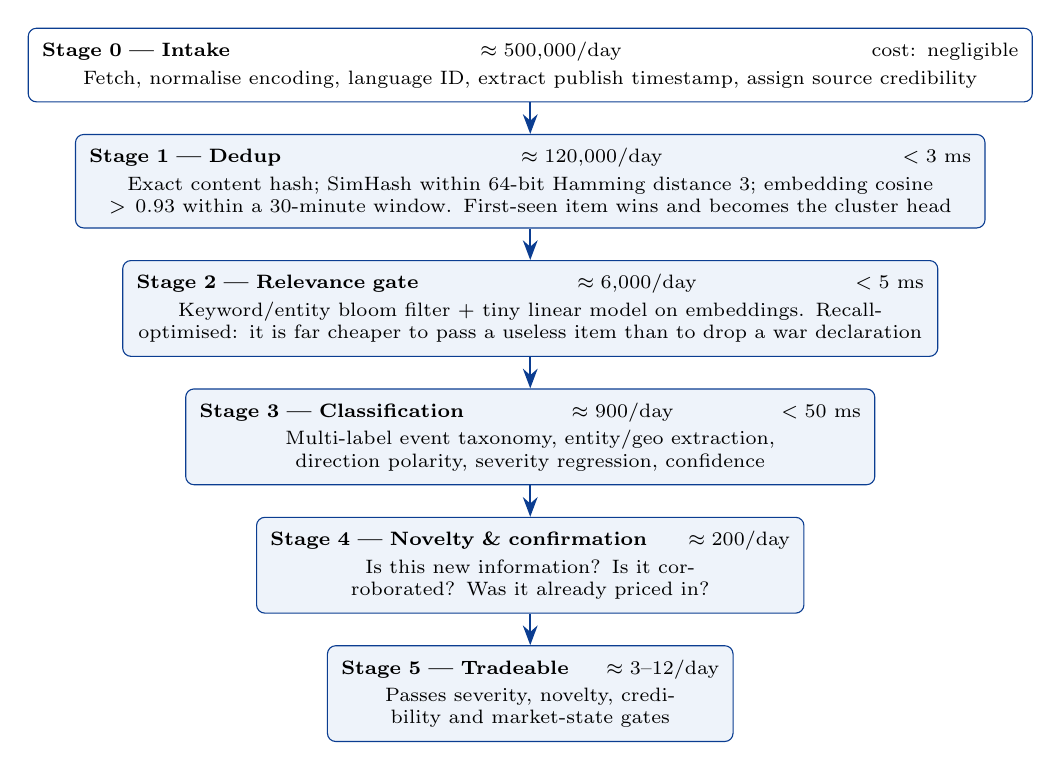
\begin{tikzpicture}[node distance=4mm]
\node[wide,text width=12.4cm,fill=white] (s0) {\textbf{Stage 0 --- Intake} \hfill $\approx 500{,}000$/day \hfill cost: negligible\\[2pt]
\scriptsize Fetch, normalise encoding, language ID, extract publish timestamp, assign source credibility};
\node[wide,text width=11.2cm,below=of s0] (s1) {\textbf{Stage 1 --- Dedup} \hfill $\approx 120{,}000$/day \hfill $<3$ ms\\[2pt]
\scriptsize Exact content hash; SimHash within 64-bit Hamming distance 3; embedding cosine $>0.93$ within a 30-minute window. First-seen item wins and becomes the cluster head};
\node[wide,text width=10.0cm,below=of s1] (s2) {\textbf{Stage 2 --- Relevance gate} \hfill $\approx 6{,}000$/day \hfill $<5$ ms\\[2pt]
\scriptsize Keyword/entity bloom filter + tiny linear model on embeddings. Recall-optimised: it is far cheaper to pass a useless item than to drop a war declaration};
\node[wide,text width=8.4cm,below=of s2] (s3) {\textbf{Stage 3 --- Classification} \hfill $\approx 900$/day \hfill $<50$ ms\\[2pt]
\scriptsize Multi-label event taxonomy, entity/geo extraction, direction polarity, severity regression, confidence};
\node[wide,text width=6.6cm,below=of s3] (s4) {\textbf{Stage 4 --- Novelty \& confirmation} \hfill $\approx 200$/day\\[2pt]
\scriptsize Is this new information? Is it corroborated? Was it already priced in?};
\node[wide,text width=4.8cm,below=of s4] (s5) {\textbf{Stage 5 --- Tradeable} \hfill $\approx 3$--$12$/day\\[2pt]
\scriptsize Passes severity, novelty, credibility and market-state gates};
\draw[ar](s0)--(s1); \draw[ar](s1)--(s2); \draw[ar](s2)--(s3); \draw[ar](s3)--(s4); \draw[ar](s4)--(s5);
\end{tikzpicture}
\end{center}

\begin{keybox}[title={Asymmetric error policy}]
Stages 0--2 are tuned for \textbf{recall} (never lose a real event). Stages 3--5
are tuned for \textbf{precision} (never trade a non-event). Mixing these
objectives in one model is the classic mistake.
\end{keybox}

\section{Event taxonomy}

The taxonomy is the backbone of the entire system: impact priors, features,
model conditioning and post-trade attribution are all keyed on it. It must be
designed once, carefully, and versioned.

\begin{longtable}{@{}p{3.3cm}p{4.4cm}p{2.1cm}p{4.4cm}@{}}
\toprule
\textbf{Family} & \textbf{Classes (examples)} & \textbf{Typical\newline severity}
& \textbf{Primary Indian transmission channel}\\
\midrule
\endhead
Monetary policy & rate decision, stance change, liquidity measure, unscheduled
action, minutes/commentary & 6--10 & Bank Nifty directly; rate-sensitive
sectors; currency\\
Macro release & inflation, growth, employment, trade balance, industrial output,
fiscal data & 4--8 & Broad index via surprise vs consensus\\
Geopolitical & military action, escalation rhetoric, territorial incident,
sanctions, treaty, coup & 3--10 & Risk premium, crude, currency, gold; defence
and oil-marketing sectors\\
Trade \& tariffs & tariff announcement, export ban, supply-chain restriction &
4--9 & Export sectors (IT, pharma, chemicals, textiles)\\
Energy & production quota change, supply disruption, strategic reserve action,
pipeline/refinery incident & 4--9 & Crude to inflation to rates; paint,
aviation, oil marketing, tyres\\
Domestic policy & budget item, regulatory change, sector reform, tax change,
subsidy & 3--9 & Sector-specific, occasionally index-wide\\
Corporate/market structure & index rebalancing, large block deal, big listing,
margin/regulatory change & 3--7 & Flow-driven, highly mechanical, often the most
predictable class\\
Flows \& positioning & foreign flow reversal, large open-interest shift,
expiry-day pinning & 3--6 & Mechanical, intraday, exploitable\\
Disaster \& health & natural disaster, epidemic, major infrastructure failure &
2--9 & Insurance, infrastructure, supply chains\\
Political & election result, coalition change, major resignation, scandal &
3--10 & Broad risk premium; extremely high variance\\
Noise / non-event & opinion, analysis, repetition, speculation & 0--2 &
\textbf{Explicit class} --- the model must learn to say ``nothing here''\\
\bottomrule
\end{longtable}

Each classified event carries the following fields.

\begin{longtable}{@{}p{3.2cm}p{2.4cm}p{9.0cm}@{}}
\toprule
\textbf{Field} & \textbf{Type} & \textbf{Meaning and how it is produced}\\
\midrule
\texttt{class}, \texttt{subclass} & enum & Multi-label transformer classifier.\\
\texttt{polarity} & $[-1,1]$ & Risk-off ($-1$) to risk-on ($+1$) for Indian
equities specifically --- \emph{not} generic sentiment. A rate cut is negative
sentiment about growth but positive polarity for equities.\\
\texttt{severity} & $[0,10]$ & Regression head trained on human-labelled
anchors; described in Section~\ref{sec:severity}.\\
\texttt{confidence} & $[0,1]$ & Classifier probability, temperature-calibrated.\\
\texttt{entities} & list & Countries, institutions, commodities, companies,
sectors --- linked to a canonical knowledge graph, not free text.\\
\texttt{geo} & list & Location plus a distance/exposure weight to India.\\
\texttt{novelty} & $[0,1]$ & Section~\ref{sec:novelty}.\\
\texttt{credibility} & $[0,1]$ & Source weight, boosted by corroboration.\\
\texttt{surprise} & $\mathbb{R}$ & For scheduled events: $(\text{actual} -
\text{consensus})/\sigma_{\text{consensus}}$. Null otherwise.\\
\texttt{expected} & bool & Was this event on the calendar? Scheduled and
unscheduled events behave completely differently.\\
\bottomrule
\end{longtable}

\section{Severity: how to make it real and not arbitrary}
\label{sec:severity}

A hand-written severity table will not survive contact with reality. Build
severity in three passes:

\begin{enumerate}
\item \term{Anchor set.} Hand-label 400--600 historical headlines on a 0--10
scale using written rubrics with concrete anchors (10 = existential shock;
7 = major unexpected policy shift; 4 = meaningful but priced; 1 = commentary).
Two labellers, measure inter-annotator agreement, resolve disagreements.
\item \term{Supervised head.} Train a regression head on the encoder to predict
the anchor scores.
\item \term{Empirical recalibration.} This is the step everyone skips: regress
the predicted severity against the \emph{realised} absolute abnormal move of
Nifty in the following 30 minutes across all historical events. Then remap
severity so that it is monotonic in realised impact. Severity becomes an
\emph{empirically grounded} quantity rather than an opinion.
\end{enumerate}

\[
\text{severity}^{\text{cal}} = F^{-1}_{|r_{30}|}\!\left(
\hat{F}_{\text{sev}}\big(\text{severity}^{\text{raw}}\big)\right)
\]
where $\hat F_{\text{sev}}$ is the empirical CDF of raw severity and
$F_{|r_{30}|}$ the empirical CDF of absolute 30-minute abnormal returns.

\section{Novelty: is this actually new information?}
\label{sec:novelty}

The most expensive mistake is trading a re-report of something already priced.
Novelty combines four signals:

\begin{align*}
\text{novelty} \;=\;\;& w_1 \underbrace{\big(1-\max_j \cos(e, e_j)\big)}_{\text{semantic distance to last 6 h}}
\;+\; w_2 \underbrace{\mathbb{1}[\text{first mention in cluster}]}_{\text{primacy}} \\[5pt]
+\;& w_3 \underbrace{(1 - \rho_{\text{cal}})}_{\text{not on calendar}}
\;+\; w_4 \underbrace{\big(1 - |\hat r_{\text{pre}}| / \sigma_{5}\big)}_{\text{market has not already moved}}
\end{align*}

The fourth term is the most underrated: if the index has already moved two
standard deviations in the five minutes \emph{before} our detection, the
information is in the price and the opportunity has passed. In that case the
system should consider a \emph{fade} strategy or, more usually, no trade at all.

\section{Confirmation and the fake-news defence}

\begin{longtable}{@{}p{3.4cm}p{5.2cm}p{5.8cm}@{}}
\toprule
\textbf{Rule} & \textbf{Condition} & \textbf{Consequence}\\
\midrule
Single low-credibility source & $c < 0.5$, no corroboration & Hot-lane alert
only. No directional signal. Volatility-widening only.\\
Corroboration window & Second independent source with $c \ge 0.75$ within 120 s
& Credibility upgraded; directional signal permitted.\\
Official confirmation & Primary source (regulator, central bank, exchange,
official channel) & Full weight immediately.\\
Contradiction & An equally credible source contradicts within 5 min & Emit
\texttt{RETRACTION}; immediately close any position opened on that event and
mark the event poisoned.\\
Extreme severity gate & severity $\ge 9$ & Requires \textbf{two} independent
sources with $c \ge 0.8$ regardless of speed. The most extreme headlines are the
most likely to be fake.\\
Market disagreement & Signal says down, but index, futures and currency all move
up within 30 s & Suppress. The market is a better classifier than we are.\\
\bottomrule
\end{longtable}

\begin{warnbox}[title={The AP-hack test}]
Before going live, run this test: inject a synthetic, highly credible-looking
but false catastrophic headline from a single medium-credibility source into a
replay. \textbf{The system must not produce a directional trade.} If it does,
the confirmation logic is wrong. Repeat this test in CI forever.
\end{warnbox}

\section{Entity-to-instrument routing}

An event mentioning ``crude supply disruption'' must mechanically become an
exposure vector. Maintain a knowledge graph:

\begin{lstlisting}[language=Python,caption={Exposure routing (conceptual)}]
# knowledge graph edge: (entity) --affects--> (factor) --loads_on--> (instrument)
EXPOSURE = {
    "crude_oil": {"NIFTY": -0.25, "BANKNIFTY": -0.15,
                  "sector:OIL_MKTG": -0.80, "sector:AVIATION": -0.70,
                  "sector:PAINTS": -0.55, "sector:UPSTREAM": +0.60},
    "usd_inr_up": {"NIFTY": -0.20, "sector:IT": +0.65, "sector:PHARMA": +0.40},
    "rbi_rate_cut": {"BANKNIFTY": +0.70, "NIFTY": +0.45,
                     "sector:REALTY": +0.75, "sector:AUTO": +0.55},
}
# Beta values are ESTIMATED FROM HISTORY (rolling regression), never hand-typed
# in production. The dict above is only the bootstrap prior for cold start.
\end{lstlisting}

\begin{keybox}[title={Rule}]
Hand-written coefficients are acceptable only as a cold-start prior. Every
coefficient must be replaced by a rolling empirical estimate with a confidence
interval as soon as sufficient history exists. The system must be able to answer
``how do you know?'' with a number and a sample size.
\end{keybox}

% =====================================================================
\chapter{Impact Scoring Engine}
\label{ch:impact}
% =====================================================================

\section{What impact scoring actually is}

The original design computes ``Nifty will drop 1.5\%''. That is a point estimate
with no error bar, and it is the root cause of over-sizing. The correct object
is a \term{conditional predictive distribution}:

\[
P\big(r_{t \to t+h} \;\big|\; \text{event class } c,\ \text{severity } s,\
\text{surprise } z,\ \text{market state } m\big)
\]

produced primarily from historical evidence, and used as a \emph{prior} that the
ML models in Chapter~\ref{ch:ml} then update with live microstructure.

\section{Building the impact library: event study methodology}

For every historical event of class $c$:

\begin{enumerate}
\item Define the event time $t_0$ precisely (publish timestamp, exchange time).
\item Compute the \term{abnormal return} over horizon $h$: subtract the expected
return given the market's normal behaviour at that time of day and volatility
regime,
\[
AR_{h} = r_{t_0 \to t_0+h} - \hat{\mathbb{E}}\!\left[r_{h} \mid
\text{time-of-day}, \sigma_{\text{regime}}, \text{day-type}\right].
\]
Time-of-day normalisation matters enormously in Indian intraday data: the
volatility profile is strongly U-shaped, so a raw 0.3\% move at 09:20 is
ordinary while the same move at 13:30 is extreme.
\item Compute a matched \term{control distribution}: sample non-event windows
with the same time-of-day and volatility regime.
\item Record: $AR_h$ for $h \in \{1,5,15,30,60\}$ minutes, realised volatility
ratio, implied volatility change, maximum favourable and adverse excursion,
volume ratio, and time-to-peak.
\item Test significance against the control distribution with a bootstrap, not a
normal approximation (intraday returns are fat-tailed).
\end{enumerate}

\begin{longtable}{@{}p{4.0cm}p{10.6cm}@{}}
\toprule
\textbf{Stored statistic} & \textbf{Why it matters for trading}\\
\midrule
Median $AR_h$ and quantiles & The realistic expectation and its spread.\\
$P(\text{sign correct})$ & Whether a directional trade is even sensible.\\
Realised-vol ratio $\sigma_{\text{post}}/\sigma_{\text{pre}}$ & Whether to buy
volatility.\\
$\Delta\sigma_{\text{IV}}$ distribution & \textbf{The vega decision.} Determines
whether options get more or less expensive.\\
Max favourable / adverse excursion & Where to put the target and the stop, from
evidence rather than a round number.\\
Time-to-peak & The correct holding period; also determines the horizon to trade.\\
Half-life of the effect & Whether the move persists or mean-reverts.\\
Sample size $n$ & The honesty check.\\
\bottomrule
\end{longtable}

\section{Hierarchical Bayesian shrinkage for rare events}

Most interesting events are rare. With $n=4$ historical instances, the empirical
mean is noise. Use a hierarchical model that shrinks class-level estimates
toward their family-level estimate:

\[
\mu_c \sim \mathcal{N}(\mu_{\text{family}}, \tau^2), \qquad
AR_{c,i} \sim \mathcal{N}(\mu_c \cdot g(s_i), \sigma_c^2)
\]

with posterior mean approximately
\[
\hat\mu_c = \frac{n_c/\sigma_c^2}{n_c/\sigma_c^2 + 1/\tau^2}\,\bar{AR}_c
\;+\; \frac{1/\tau^2}{n_c/\sigma_c^2 + 1/\tau^2}\,\mu_{\text{family}} .
\]

\begin{keybox}[title={Practical consequence}]
With $n_c = 3$, the estimate is dominated by the family prior --- which is
exactly correct behaviour. The engine reports the posterior \emph{and} the
sample size, and the risk gate reduces position size when the posterior variance
is high. Refuse to emit a class-specific impact when $n_c < 8$ and no family
prior exists; fall back to ``unknown event, volatility-only response''.
\end{keybox}

\section{The live scoring formula}

\[
\hat{r}_h \;=\; \underbrace{\hat\mu_{c,h}}_{\text{Bayesian prior}}
\times \underbrace{g(s)}_{\text{severity}}
\times \underbrace{\nu}_{\text{novelty}}
\times \underbrace{c_{\text{cred}}}_{\text{credibility}}
\times \underbrace{\kappa(m)}_{\text{regime}}
\times \underbrace{\lambda(\tau)}_{\text{time-of-day}}
\times \underbrace{(1-\pi)}_{\text{already-priced discount}}
\]

\begin{longtable}{@{}p{2.2cm}p{4.0cm}p{8.4cm}@{}}
\toprule
\textbf{Term} & \textbf{Form} & \textbf{Notes}\\
\midrule
$g(s)$ & $\left(s/5\right)^{\gamma}$, $\gamma \approx 1.4$ fitted &
Impact is convex in severity: a 9 is much more than twice a 4.5.\\
$\nu$ & novelty score & Old news gets multiplied toward zero.\\
$c_{\text{cred}}$ & credibility & Unconfirmed rumour is heavily discounted.\\
$\kappa(m)$ & regime multiplier & Same event has larger impact in a
high-volatility, low-liquidity regime. Fitted per regime cluster.\\
$\lambda(\tau)$ & time-of-day multiplier & U-shaped; also handles the special
cases of the opening 15 minutes, the pre-close and expiry-day afternoons.\\
$\pi$ & $\min\!\big(1, |r_{\text{pre}}| / |\hat\mu_{c,h}|\big)$ &
If the market has already made the expected move before we act, the remaining
opportunity is gone. \textbf{This term is what prevents chasing.}\\
\bottomrule
\end{longtable}

The output is not a scalar but a triple: $(\hat r_h,\ \text{quantiles},\
n_{\text{eff}})$ for each horizon $h$, plus a separate volatility forecast
$(\hat\sigma_{\text{post}}/\sigma_{\text{pre}},\ \widehat{\Delta\sigma_{IV}})$.

\section{Cross-asset propagation}

When an event occurs outside Indian market hours, or affects a foreign asset
first, the impact reaches Nifty through a measurable chain. Estimate the chain
empirically with lagged regressions and store the transfer coefficients:

\begin{longtable}{@{}p{3.6cm}p{3.2cm}p{7.8cm}@{}}
\toprule
\textbf{Channel} & \textbf{Typical lag} & \textbf{Modelling note}\\
\midrule
GIFT/SGX Nifty to Nifty spot & Near-instant during overlap; sets the gap when
Indian market is shut & The single most useful overnight variable.\\
US equity futures to Indian open & Overnight & Estimate a gap model:
$r_{\text{gap}} = \alpha + \beta\, r_{\text{US futures}} + \ldots$\\
Crude to Nifty & Minutes to hours & Asymmetric: sharp spikes transmit faster
than slow drifts.\\
USD/INR to Nifty & Minutes & Bidirectional causality; use a vector
autoregression, not a simple regression.\\
US Treasury yields to Bank Nifty & Hours & Slower; more relevant to the next
session.\\
Asian indices to Nifty intraday & Minutes & Useful during the 09:15--12:00
window.\\
\bottomrule
\end{longtable}

\begin{keybox}[title={The overnight opportunity}]
Roughly half of the total price change in Indian indices arrives as overnight
gaps. Most retail systems ignore this because they only look at intraday
candles. A well-calibrated \term{gap forecaster} driven by overnight global
events is arguably an easier and more profitable first product than intraday
prediction --- and it needs no low-latency infrastructure at all. Consider
shipping it first (see Phase~4 in the roadmap).
\end{keybox}


\end{document}
